% !Mode:: "TeX:UTF-8"
% !TEX program  = xelatex

% \documentclass{hfutreport}
\documentclass[bwprint]{hfutreport}

\title{基于以太坊的微博系统设计与实现}
\stunum{20184347, 20181656}
\stuname{王\quad 浩, 李涵威}
\stuclass{信息安全2班, 信息安全1班}
\supervisor{叶春晓}
\dateinput{\today}

\begin{document}

\maketitle

% 目录使用Romen页脚 
\pagestyle{plain}
\pagenumbering{Roman}
\tableofcontents
\newpage
\pagestyle{plain}

%正文页脚
\setcounter{page}{1}
\pagenumbering{arabic}

\section{项目简介}
\subsection{概述}
这是一个运行在以太坊上的去中心微博系统,去中心化意味着没有一个中心化机构能够控制你发送的微博,你
发送的微博是由你完全控制的,任何人无法删除、关闭你的微博。一旦你的微博发出去后,只有你自己能删除它。

\subsection{传统微博与去中心化微博的对比}
传统微博(如新浪微博)就是一个中心化的应用平台,新浪公司就是整个微博平台的中心。新浪公司制定新浪微博
的运行规则,开发出整个微博平台,为其提供中央服务器,维持着整个新浪微博的运转,并不断地向外推广,吸引
用户使用。一切商业行为都是为了追逐利益的,新浪公司运营新浪微博,也是为了吸引广告主投放广告,从而获得
巨额的广告收入。

在中心化的微博平台中,大致流程如\cref{fig:classical-weibo}~所示,博主(发微博者)会编辑微博发送到新浪微博平台中,新浪微博将微
博推送给观众(看微博者),观众查看微博,微博中会夹杂着一些广告,观众看微博时也会看到一些广告。广告主
会为广告的浏览量和点击量,支付广告费给新浪公司。

\begin{figure}[!htbp]
    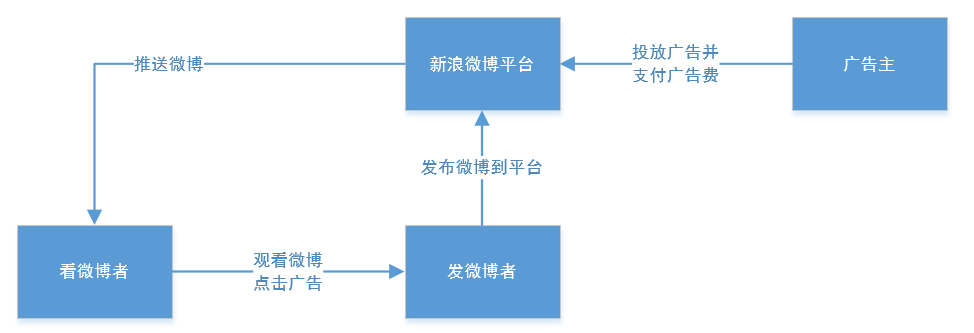
\includegraphics[width=\linewidth]{classical-weibo}
    \caption{传统中心化微博运作流程}
    \label{fig:classical-weibo}
\end{figure}

与传统微博平台不同,在去中心化微博平台中,将没有中心机构,没有中央服务器,主要是通过区块链技术,运用
分布式自治组织(DAO)的组织架构,实现微博平台的自治。让每一个微博参与者都成为微博平台的所有者,他们
将共享微博平台获得的全部收益。

\section{系统框架}
\subsection{运作流程}
该去中心化微博系统部署在以太坊区块链上,采用智能合约作为数据存储后端,采用Web前端提供用户操作界面。整个
系统的流程如\cref{fig:system-flow}~所示。

\begin{figure}[!htbp]
    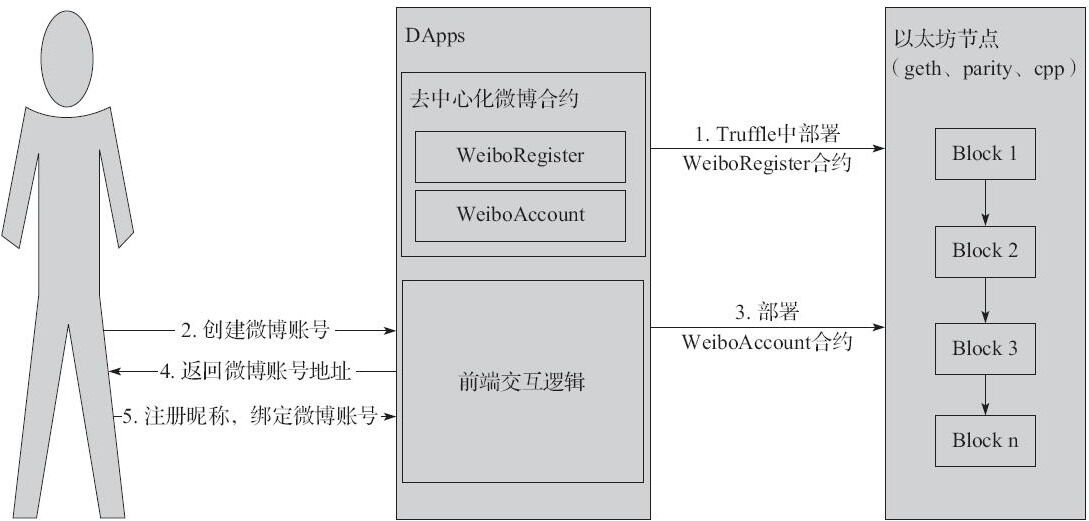
\includegraphics[width=\linewidth]{system-flow}
    \caption{去中心化微博的运作流程}
    \label{fig:system-flow}
\end{figure}

\subsection{方案选型}
\subsubsection{以太坊客户端}
在目前开发DApp去中心化应用中,Ganache和Geth这两种以太坊客户端使用较为普遍,本项目可以同时运行
部署在Ganache和Geth中。但是在测试开发中,比较推荐Ganache。Ganache是基于Node.js开发的以太坊
客户端,整个区块链的数据驻留在内存,发送给Ganache的交易会被马上处理而不需要等待挖矿时间。Ganache
可以在启动时创建一堆存有资金的测试账户,它的运行速度也更快,因此更适合开发和测试。

\subsubsection{开发框架}
本项目使用Truffle开发工具。Truffle是基于以太坊的智能合约开发工具,支持对合约代码的单元测试,非常
适合测试驱动开发。同时内置了智能合约编译器,只要使用脚本命令就可以完成合约的编译、部署、测试等工作,
大大简化了合约的开发生命周期。

\subsubsection{前端应用框架}
本项目采用Web前端,基于Webpack Truffle Box模板搭建,并使用了jQuery和Bootstrap框架简化前端
页面的开发。

\subsection{总体设计}
本系统底层使用以太坊区块链,用户在浏览器中使用MetaMask连接以太坊就可以完成所有操作,系统架构
如\cref{fig:system-arch}~所示。

\begin{figure}[!htbp]
    
\includegraphics[width=\linewidth]{system-arch}
    \caption{系统架构}
    \label{fig:system-arch}
\end{figure}


\section{功能说明}
本系统的核心业务围绕微博展开,其中用户可以发送微博,其他用户可以查看该微博并决定是否点赞或者点踩。
系统管理员可以查看所有用户信息,例如用户的微博总数、点赞总数、点踩总数等。

本系统主要涉及两类用户:微博用户和管理员。各用户的功能如\cref{tab:func}~所示。从表中我们可以
看到管理员除了查询系统信息外不具有其他功能,所以简单起见我们没有在系统中特别设立管理管,任何用户
都可以在后台页面查看后台信息和用户列表,也就是说目前所有用户其实都拥有和管理员一样的功能。
\begin{table}[!htbp]
    \caption{用户功能}\label{tab:func}
    \centering
    \begin{tabular}{ccl}
        \hline
        \textbf{}                 & \textbf{需求要点} & \textbf{备注}                                        \\ \hline
        \multirow{6}{*}{微博用户} & 注册              & 使用以太坊账户注册一个微博账户,并指定一个唯一的昵称 \\
                                  & 登录              & 使用以太坊账户进行登录,一般由MetaMask自动完成       \\
                                  & 查询              & 用户查询自己的个人信息,包括ID、昵称、历史微博等     \\
                                  & 发微博              & 用户可以发送一条新的微博     \\
                                  & 点赞              & 用户可以对首页看到的其他用户的微博进行点赞           \\
                                  & 点踩              & 用户可以对首页看到的其他用户的微博进行点踩           \\ \hline
        管理员                    & 查询              & 管理员可以查看完整的用户列表、微博总数等系统信息     \\ \hline
    \end{tabular}
\end{table}

\section{设计思路}

\subsection{创建项目}
前面我们已经介绍过本项目的方案选型,我们在开发环境中使用Ganache作为以太坊客户端进行智能合约的
部署,同时使用Truffle作为开发框架构建我们的项目。简化起见,我们不使用React项目模板,而使用
Webpack项目模板,这样我们使用传统的前端开发技术完成前端页面的编写。
\begin{lstlisting}[language=bash]
# 安装 Truffle
npm install -g truffle
# 创建项目目录
mkdir dapp-weibo
cd dapp-weibo
# 拉取项目模板创建新项目
truffle unbox webpack
\end{lstlisting}

项目创建好后目录结构如下:
\begin{verbatim}
    |--app --------------------前端项目
    |--|--src -----------------网页源码html\css\javascript
    |--contracts --------------智能合约
    |--migrations -------------合约部署脚本
    |--test -------------------合约测试脚本    
\end{verbatim}

\newpage
之后我们使用下面这些命令完成项目的构建、部署、测试、启动等:
\begin{lstlisting}[language=bash]
# 编译智能合约
truffle compile
# 部署智能合约
truffle migrate
# 测试智能合约
truffle test
# 启动前端
cd app && npm run dev
# 构建前端
cd app && npm run build
\end{lstlisting}

\subsection{合约}
\subsubsection{数据结构}
我们需要在合约中存储用户信息和微博信息,我们将其分别定义为一个结构体,其中微博结构体需要存储
微博创建的时间戳、微博内容、点赞数量和点踩数量,微博用户结构体需要存储用户ID、用户账户地址、
用户名、微博数量、所有微博。具体定义如下:

\begin{lstlisting}[language=c]
// 博文
struct Blog {
    uint256 timestamp;
    string content;
    bool isValid;
    uint256 like;
    uint256 dislike;
}

// 微博用户
struct User {
    uint256 id;
    address addr;
    string name;
    bool isValid;
    uint256 blogNumber;
    mapping(uint256 => Blog) blogs;
}
\end{lstlisting}

同时为了方便我们在合约方法中通过账户地址、用户ID、用户名等各种不同的方式查询用户,
我们定义了下面几个映射表:

\begin{lstlisting}[language=c]
// 存储用户的hash表
mapping(address => User) users;
mapping(address => string) address2name;
mapping(string => address) name2address;
mapping(uint256 => address) id2address;
\end{lstlisting}

\subsubsection{合约方法}
创建一个微博用户时需要检测该用户昵称是否被占用以及该账户地址是否以及注册,如果出现昵称占用或者
账户以及被注册则提示注册失败,反之则在\verb|users|映射表中新建一个微博用户,同时维护好所有
映射关系。具体实现如下:

\begin{lstlisting}[language=c]
// 创建用户
event CreateUser(address sender, bool isSuccess, string message);

function createUser(string memory name) public {
    // name已经被占用
    if (name2address[name] != address(0)) {
        emit CreateUser(msg.sender, false, "昵称已被占用");
        return;
    }
    // msg.sender 已经注册过
    if (bytes(address2name[msg.sender]).length != 0) {
        emit CreateUser(msg.sender, false, "您的账户已被注册");
        return;
    }
    // 昵称长度超过64字节限制
    if (bytes(name).length == 0 || bytes(name).length > 64) {
        emit CreateUser(msg.sender, false, "昵称长度不合理");
        return;
    }
    users[msg.sender].id = userNumber;
    users[msg.sender].addr = msg.sender;
    users[msg.sender].name = name;
    users[msg.sender].blogNumber = 0;
    users[msg.sender].isValid = true;
    // 保存id到账户的映射关系
    id2address[userNumber] = msg.sender;
    // 保存账户到昵称的双向映射关系
    address2name[msg.sender] = name;
    name2address[name] = msg.sender;
    userNumber++;
    emit CreateUser(msg.sender, true, "新用户创建成功");
}
\end{lstlisting}

发微博时需要检测博文长度是否超过限制,如果超过限制则提示发送失败,否则在对应用户的\verb|blogs|
映射表中新建一条微博,同时需要将微博的点赞数和点踩数都置为0。具体实现如下:
\begin{lstlisting}[language=c]
// 发微博
event PostBlog(address sender, bool isSuccess, string message);

function postBlog(string memory content) public {
    // 微博长度超过160字节
    if (bytes(content).length == 0 || bytes(content).length > 160) {
        emit PostBlog(msg.sender, false, "博文长度不合理");
        return;
    }
    users[msg.sender].blogs[users[msg.sender].blogNumber].timestamp = now;
    users[msg.sender].blogs[users[msg.sender].blogNumber].content = content;
    users[msg.sender].blogs[users[msg.sender].blogNumber].like = 0;
    users[msg.sender].blogs[users[msg.sender].blogNumber].dislike = 0;
    users[msg.sender].blogs[users[msg.sender].blogNumber].isValid = true;
    users[msg.sender].blogNumber++;
    emit PostBlog(msg.sender, true, "微博发布成功");
}
\end{lstlisting}

给指定用户的指定微博点赞/点踩时需要将用户ID和微博ID传给合约方法,方法中检测该用户的该微博
是否存在如果不存在则提示失败,反之给该微博的点赞数/点踩数增加1。具体实现如下:
\begin{lstlisting}[language=c]
// 给博文点赞
event LikeBlog(address sender, bool isSuccess, string message);

function likeBlog(uint256 user_id, uint256 blog_id) public {
    address addr = id2address[user_id];
    if (!users[addr].isValid) {
        emit LikeBlog(msg.sender, false, "用户不存在");
        return;
    }
    if (!users[addr].blogs[blog_id].isValid) {
        emit LikeBlog(msg.sender, false, "博文不存在");
        return;
    }
    users[addr].blogs[blog_id].like += 1;
    emit LikeBlog(msg.sender, true, "点赞成功");
}

// 给博文点踩
event DislikeBlog(address sender, bool isSuccess, string message);
function dislikeBlog(uint256 user_id, uint256 blog_id) public {
    address addr = id2address[user_id];
    if (!users[addr].isValid) {
        emit LikeBlog(msg.sender, false, "用户不存在");
        return;
    }
    if (!users[addr].blogs[blog_id].isValid) {
        emit LikeBlog(msg.sender, false, "博文不存在");
        return;
    }
    users[addr].blogs[blog_id].dislike += 1;
    emit LikeBlog(msg.sender, true, "点踩成功");
}
\end{lstlisting}

当然为了前端能够很好的给用户展示用户的个人信息,用户的微博列表,系统的用户列表等信息,我们
还需要在合约中提供一系列的查询方法,例如查询用户总数、查询博文总数、根据用户ID查询用户信息、
根据用户ID和微博ID查询微博等。由于大部分查询都是简单的将信息返回而已,所以下面不再一一列出。
其中根据用户ID查询用户信息的方法如下:
\begin{lstlisting}[language=c]
// 根据id返回是否查询成功、昵称、账户、博文数、like、dislike
function getUserInfo(uint256 id)
    public view returns (
        bool isSuccess,
        string memory name,
        address addr,
        uint256 blogNumber,
        uint256 like,
        uint256 dislike
    ){
    if (id2address[id] == address(0)) {
        return (false, "", address(0), 0, 0, 0);
    }
    address _addr = id2address[id];
    uint256 _like = 0;
    uint256 _dislike = 0;
    for (uint256 i = 0; i < users[_addr].blogNumber; i++) {
        _like += users[_addr].blogs[i].like;
        _dislike += users[_addr].blogs[i].dislike;
    }
    return (true, users[_addr].name, users[_addr].addr, users[_addr].blogNumber, _like, _dislike);
}
\end{lstlisting}

根据用户ID和微博ID查询微博信息的方法如下:
\begin{lstlisting}[language=c]
// 根据用户id和博文id返回博文信息
function getBlog(uint256 user_id, uint256 blog_id)
    public view returns (
        bool isSuccess,
        uint256 timestamp,
        string memory content,
        uint256 like,
        uint256 dislike
    ){
    address addr = id2address[user_id];
    if (!users[addr].isValid || !users[addr].blogs[blog_id].isValid) {
        return (false, 0, "", 0, 0);
    }
    Blog memory blog = users[addr].blogs[blog_id];
    return (true, blog.timestamp, blog.content, blog.like, blog.dislike);
}
\end{lstlisting}

\subsection{前端应用}
前端页面的展示我们放在下一节进行,我们这里只对JavaScript脚本中关键的函数进行说明。首先是注册用户,
注册用户需要用户在前端页面中指定一个昵称,我们需要获取用户输入的昵称并使用Web3.js提供的API调用合
约中的\verb|createUser|方法进行用户注册,该方法的调用会主动唤起MetaMask发起一次转账,当然需要
用户手动确认。具体实现如下:

\begin{lstlisting}[language=c]
// 创建用户
createUser: async function () {
    const username = $("#inputUsername").val();
    if (username.length > 0 && username.length <= 64) {
        await this.weibo.methods.createUser(username).send({ from: this.account });
        this.weibo.events.CreateUser(function (error, event) {
        if (!error && event.returnValues.isSuccess) {
            console.log("注册账户成功");
        }
        else if (!error && !event.returnValues.isSuccess) {
            alert("账户注册失败: " + event.returnValues.message);
        }
        });
        // 清空输入框
        $("#inputUsername").val("");
        this.refreshHome();
        this.refreshMy();
        this.refreshAdmin();
    }
}
\end{lstlisting}

发微博时读取用户输入的微博内容,然后调用智能合约的\verb|postBlog|方法发送微博,具体实现如下:
\begin{lstlisting}[language=c]
// 发微博
postBlog: async function () {
    const content = $("#newBlogContent").val();
    if (content.length > 0 && content.length <= 160) {
    await this.weibo.methods.postBlog(content).send({ from: this.account });
    this.weibo.events.PostBlog(function (error, event) {
        if (!error && event.returnValues.isSuccess) {
        console.log("微博发送成功");
        }
        else if (!error && !event.returnValues.isSuccess) {
        alert("微博发送失败: " + event.returnValues.message);
        }
    });
    // 清空输入框
    $("#newBlogContent").val("");
    this.refreshHome();
    this.refreshMy();
    this.refreshAdmin();
    }
}
\end{lstlisting}

点赞和点踩同理,直接调用合约中对应的方法即可,具体实现如下:
\begin{lstlisting}[language=c]
// 点赞
like: async function (likeBtn) {
    const user_id = parseInt($(likeBtn).attr("user_id"));
    const blog_id = parseInt($(likeBtn).attr("blog_id"));
    await this.weibo.methods.likeBlog(user_id, blog_id).send({from: this.account});
    this.refreshHome();
    this.refreshMy();
    this.refreshAdmin();
},

// 点踩
dislike: async function (dislikeBtn) {
    const user_id = parseInt($(dislikeBtn).attr("user_id"));
    const blog_id = parseInt($(dislikeBtn).attr("blog_id"));
    await this.weibo.methods.dislikeBlog(user_id, blog_id).send({from: this.account});
    this.refreshHome();
    this.refreshMy();
    this.refreshAdmin();
},
\end{lstlisting}

限于篇幅,其余获取用户信息和系统信息的函数这里不再一一列举。

\section{结果展示}
首先我们启动Ganache,在终端执行\verb|ganache-cli|命令,如\cref{fig:ganache}~所示,可以看到
Ganache在\verb|127.0.0.1:8545|上开启了HTTP RPC,并且默认创建了10个账户,每个账户都有100ETH的余额。

\begin{figure}[!htbp]
    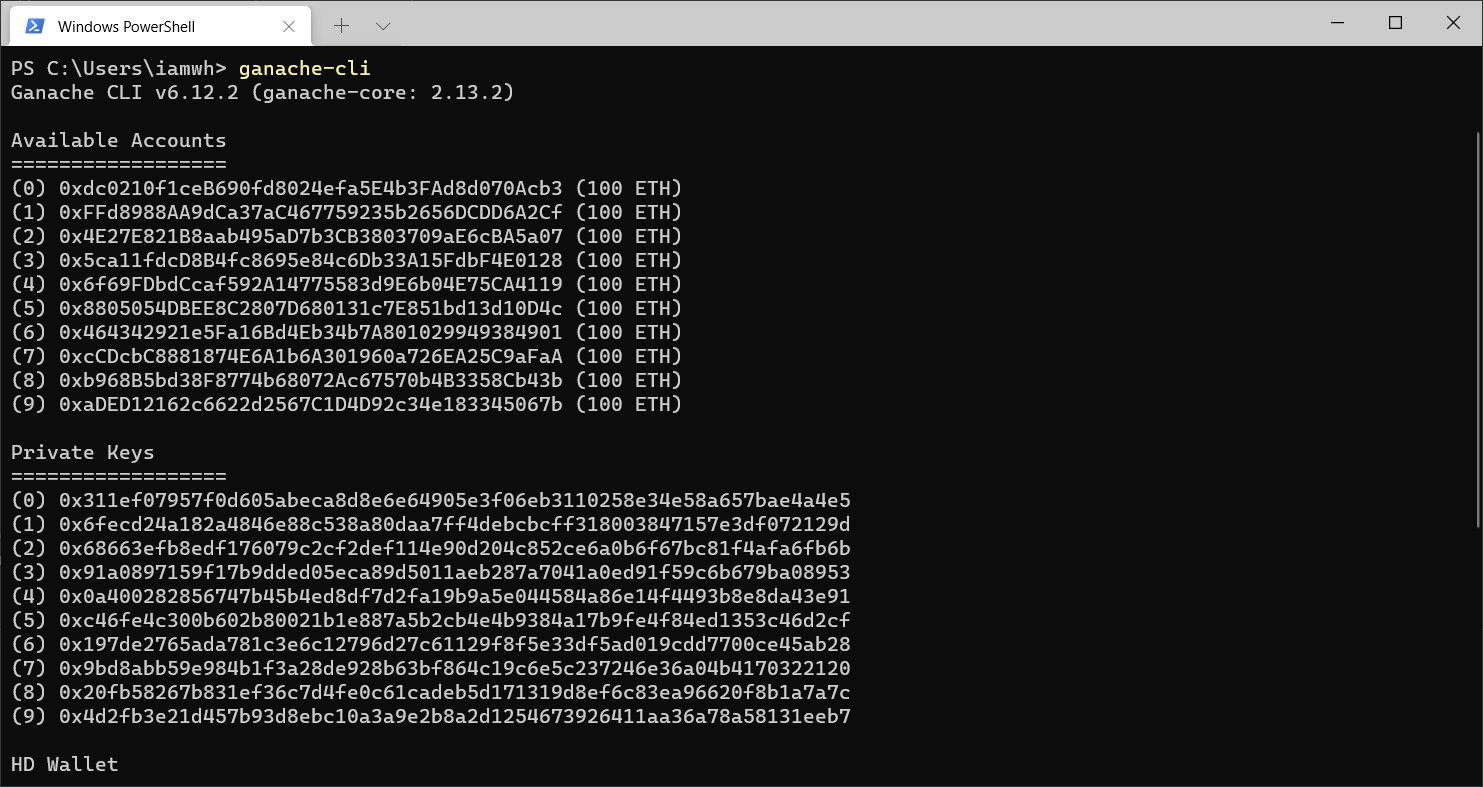
\includegraphics[width=\linewidth]{ganache}
    \caption{启动Ganache}
    \label{fig:ganache}
\end{figure}

然后我们使用\verb|truffle migrate|部署智能合约,如\cref{fig:migrate}~所示,从控制台输出中
可以得到部署完成后的合约地址为\verb|0xD1EC0F2e1E3916301068A638864990F9A2994e55|。

\begin{figure}[!htbp]
    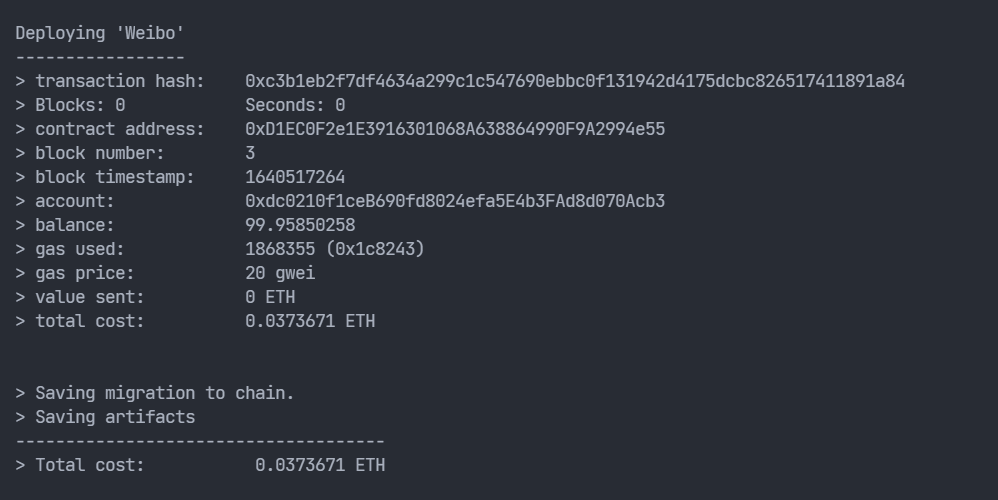
\includegraphics[width=\linewidth]{migrate}
    \caption{部署智能合约}
    \label{fig:migrate}
\end{figure}

使用\verb|cd app && npm run dev|启动Web前端,可以看到总共有三个页面:首页、用户、后台。其中首页
根据时间顺序展示了所有微博,用户可以对每一条微博点赞或者点踩,如\cref{fig:home}~所示。

\begin{figure}[!htbp]
    \centering
    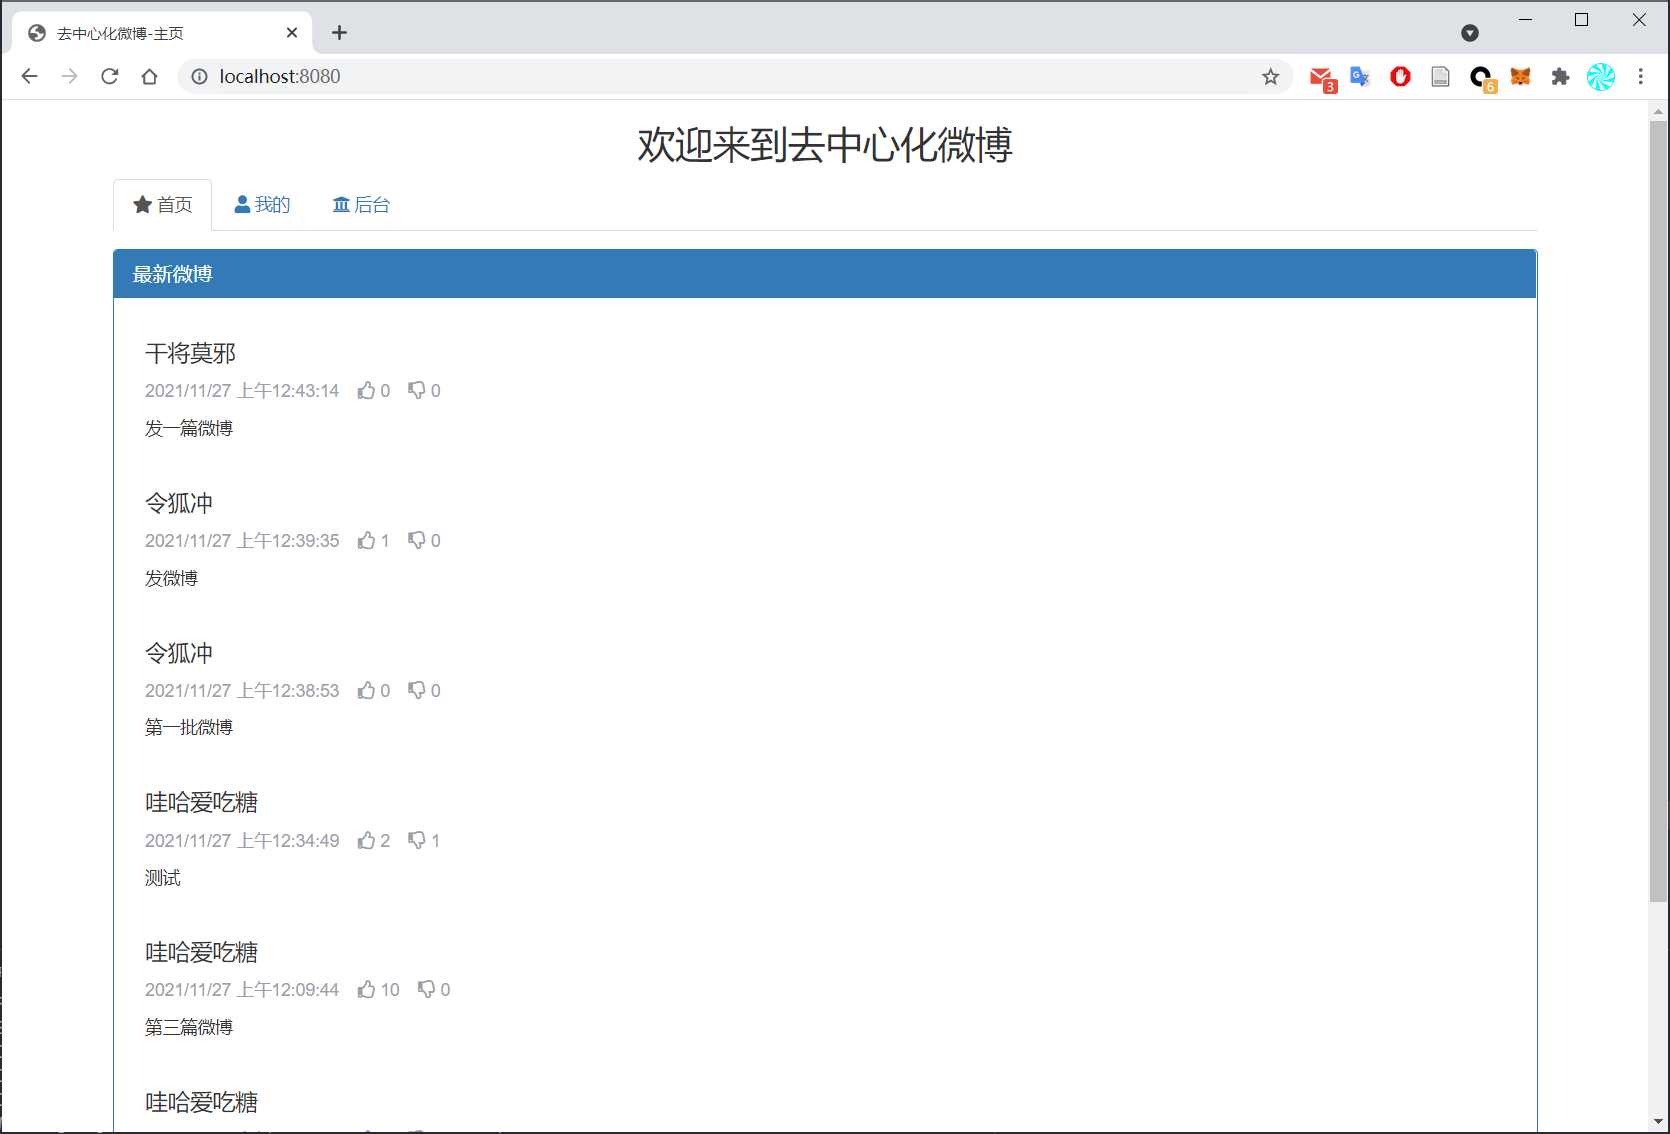
\includegraphics[width=.8\linewidth]{home}
    \caption{首页}
    \label{fig:home}
\end{figure}

用户页展示了当前用户的信息,以及发过的所有微博,当然用户也可以在这里发微博,如\cref{fig:user}~所示。

\begin{figure}[!htbp]
    \centering
    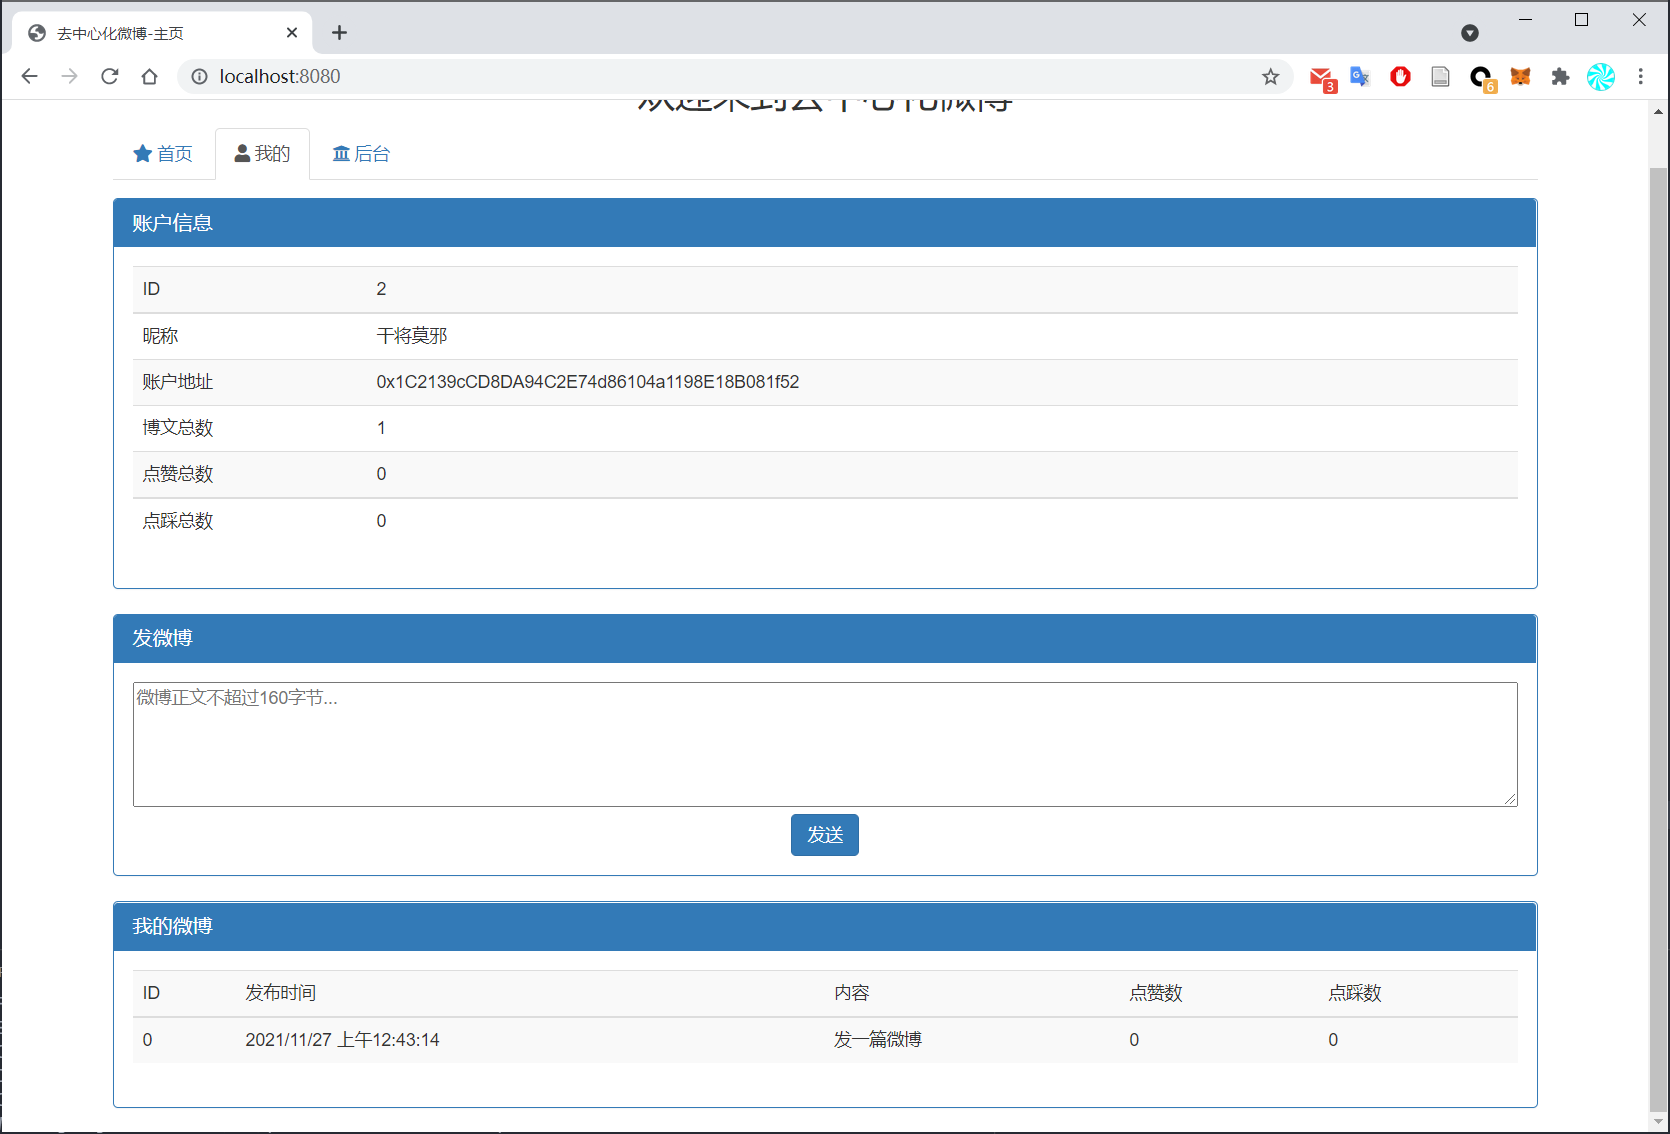
\includegraphics[width=.8\linewidth]{user}
    \caption{用户页面}
    \label{fig:user}
\end{figure}

\newpage
管理员页展示了系统信息,以及所有注册用户信息,并且可以在这个页面注册新用户,如\cref{fig:admin}~所示。

\begin{figure}[!htbp]
    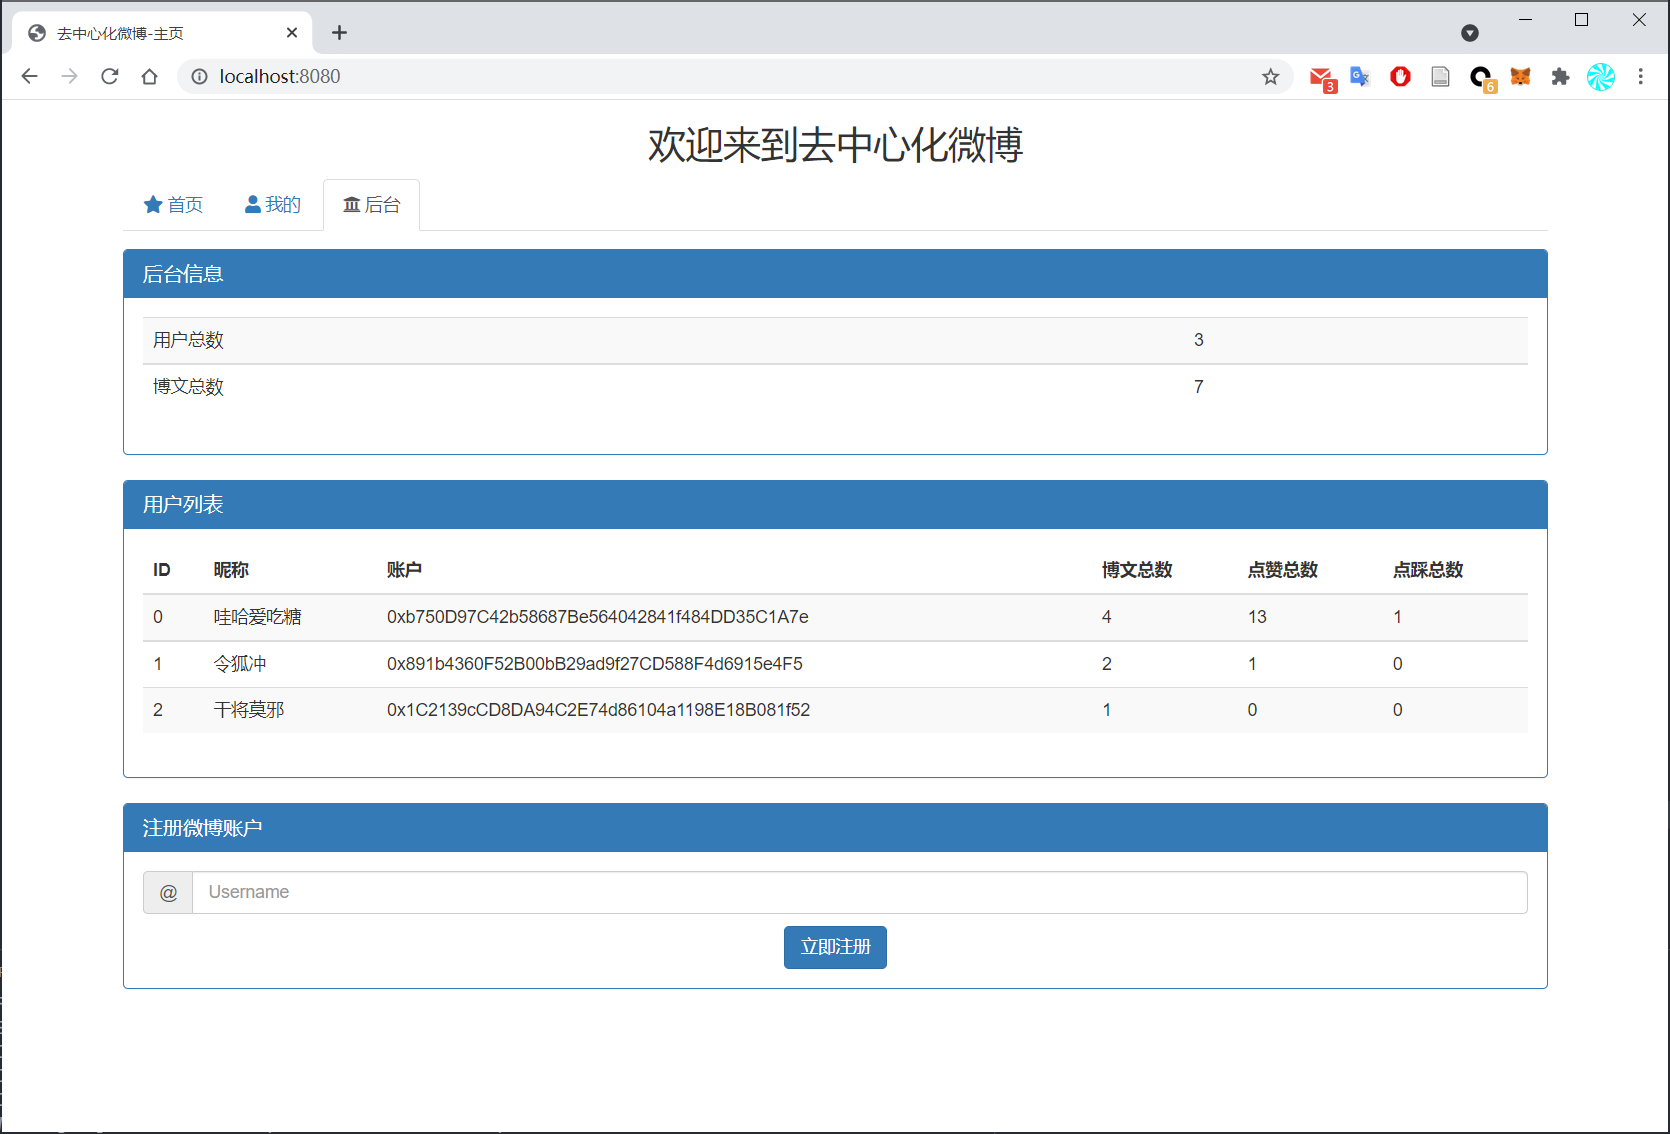
\includegraphics[width=\linewidth]{admin}
    \caption{管理员页面}
    \label{fig:admin}
\end{figure}

\section{小组分工}
我们小组共两位成员,分工情况如\cref{tab:xzfg}~所示。另外我们在GitHub上进行项目合作,完整项目代码见
仓库\href{https://github.com/iamwhcn/dapp-weibo}{https://github.com/iamwhcn/dapp-weibo}。
\begin{table}[!htbp]
    \caption{小组分工}\label{tab:xzfg}
    \centering
    \begin{tabular}{c|c|l}
        \hline
        {\bf 姓名} & {\bf 学号} & {\bf 分工}         \\
        \hline
        王\quad 浩 & 20184347  & 系统设计、合约编写、前端应用编写、报告编写 \\
        \hline
        李涵威     & 20181656   & 系统设计、合约编写、前端应用编写、演示视频录制 \\
        \hline
    \end{tabular}
\end{table}

\newpage 
\begin{thebibliography}{9}%宽度9
    \bibitem[1]{qukuailiankaifashizhan}
    吴寿鹤.
    \newblock 区块链开发实战:以太坊关键技术与案例分析[M].
    \newblock 机械工业出版社, 北京, 2018.

    \bibitem[2]{qukuailianjinjiejishushizhan}
    蔡亮.
    \newblock 区块链技术进阶与实战[M].
    \newblock 人民邮电出版社, 北京, 2018.
\end{thebibliography}


\end{document}